\subsection{Use-Cases}

Here we present two hypothetical use-cases for correspondence checking and
\simulator.

\noindent{\bf Use-Case 1: Network Operator.} An enterprise network
operator pays a third-party SDN provider to virtualize their network
and run it in the cloud. The network operator receives a complaint
from an internal team that two servers cannot reach other, and 
verifies the reachablility problem with {\tt ping}. Unsure
whether the problem is in her ACL/routing rules, 
or whether the problem is in the SDN platform, the
operator runs correspondence checking on a snapshot of the network state. She
finds that there is an inconsistency between her policy and the network state, 
and proceeds to call up the third-party SDN provider to complain
about the problem.

\noindent{\bf Use-Case 2: SDN Developer.} A developer at the third-party SDN
company receives the customer's trouble-ticket and begins to investigate the
problem. The developer examines the system logs and sees a
long list of link status events, control server reboots, VM migration events,
and other diagnostic information. These events are numerous (the
datacenter comprises 8,000 switches and more than 100,000 hosts) and
interleaved, so the developer is unsure what caused the problem.
The developer feeds a snapshot of the network from before the
trouble-ticket was issued into the simulator, and
begins replaying the execution of the system. The developer runs
correspondence checking, and finds a substantial list of inconsistencies,
manifesting as loops, blackholes, and other problems.
To isolate the root cause, the developer decides to exclude from the simulated
execution all events unrelated to the path between the two disconnected
servers. As the developer is stepping through the execution, he periodically
runs correspondence checking and tracks the inconsistencies over time. He
finds that most inconsistencies resolve within a short time. However, he
eventually encounters a blackhole which lasts a considerable time. The
developer backs up the execution to the point when consistency begins, and
observes a switch failure followed directly by a reboot of the switch's parent
controller. The developer adds log statements to the platform's failover
logic, and re-runs the execution. The developer eventually verifies that the
controller pushed a routing change to the failed switch's neighbors, but did
not update the platform's representation of the network state. Upon closer
examination, the developer finds that the new parent controller for that
portion of the network assumed that the platform's
representation of network state was up-to-date. As such, the partially installed flow entries remained
in the neighboring switches, resulting in the blackhole. The developer fixes
the platform's recovery code and pushes the change to production. The
developer also adds this case to the platform's integration test suite.
\colin{Mention correspondence checking between intermediate layers of
SDN stack?}

\subsection{Overhead}

\noindent{\bf Simulator Scalability.} We have implemented a prototype
simulator. In a single process, our prototype models hosts and OpenFlow switches 
as python objects, which communicate with a SDN controller as if they were
true hardware.

To gauge the scalability of modeling the network within a single-process,
we \colin{will have} spawned a network of 10,000 switches and measured the
time to process 5 FLOW\_MOD messages per switch. \colin{It took X seconds,
which is below the bounds of human perception}

%\tbd{Graph of simulator
%scalability. x-axis is \# of software switches. y-axis is time to process N
%OFTP\_FLOW\_MOD messages. A few lines for different values of N} \\

\noindent{\bf Record and Replay Overhead.} In contrast to general record-and-replay
mechanisms, the amount of recorded state needed for
high-fidelity replay is tractable. With proactive flow installation, 
updates are pushed to routing tables over a relatively long time scale; periodic
FIB snapshots along with a log of link state events, control server
downtime, and host mobility information suffice for our purposes. As a point of reference, the Cisco 7000 series
core switch model supports a maximum of 128K MAC entries and
128K ACL entries~\cite{cisco7000}. Assuming 36 bytes per flow entry,
(larger than OpenFlow 13-tuple), this yields
an upper bound of 9216 bytes, uncompressed, per FIB. A datacenter of 100,000
hosts includes roughly 8,000 switches~\cite{Al-Fares:2008:SCD:1402946.1402967}.
Therefore a snapshot of the FIBs of the entire network takes up roughly 74 MB.
The VL2 paper reports 36M network error events over one year over 8
datacenters, which implies 8.5 error events per minute per
datacenter~\cite{Greenberg:2009:VSF:1592568.1592576}.
Suppose we took a snapshot of the FIBs in the network every second. 
We would need then to store roughly 4GB uncompressed per minute, a relatively small growth 
rate for datacenter logs. Note that this is a conservative overestimate.
\tbd{Get numbers on frequency of VM migrations}
%To account for host mobility, assume that each server hosts 10 VMs,
%and 1\% of VMs are created, suspended, or migrated every minute. Then 10,000 host mobility events must be
%logged per minute, also a reasonable storage cost. \colin{get real numbers}

%As a point of reference, border routers' working RIB size is
%$\textasciitilde$130MB~\cite{Karpilovsky:2006:UFR:1368436.1368439}.

\noindent{\bf Correspondence Checking Runtime.} Computing the propagation
graph for correspondence checking is equivalent to enumerating
all possible paths in the network. The number of possible paths scales with the diameter
of the network as well as the number of routing entries per switch.
Each branch of the propagation graph can be
computed in parallel however, so the computation is bottlenecked by the serial runtime
of computing a single branch of the propagation graph.

We show the serial runtime of correspondence checking in 
Figure~\ref{hsa_runtime}. Each data point was generated on a single Intel Xeon
2.80GHz core. For this analysis we generated fat-tree topologies
of varying sizes, with pre-installed PORTLAND~\cite{NiranjanMysore:2009:PSF:1594977.1592575}
routing tables in each switch. Note
that the number of PORTLAND routing entries per switch scales with the number
of pods in the fat-tree. As the figure depicts, the serial runtime of
correspondence checking scales roughly quadratically with the
size of the fat-tree topology. The number of serial tasks to be executed
(total number of branches in the propagation tree) is the number of hosts
in the network squared, disregarding ECMP load-balancing.

\begin{figure}[t]
    %\hspace{-10pt}
    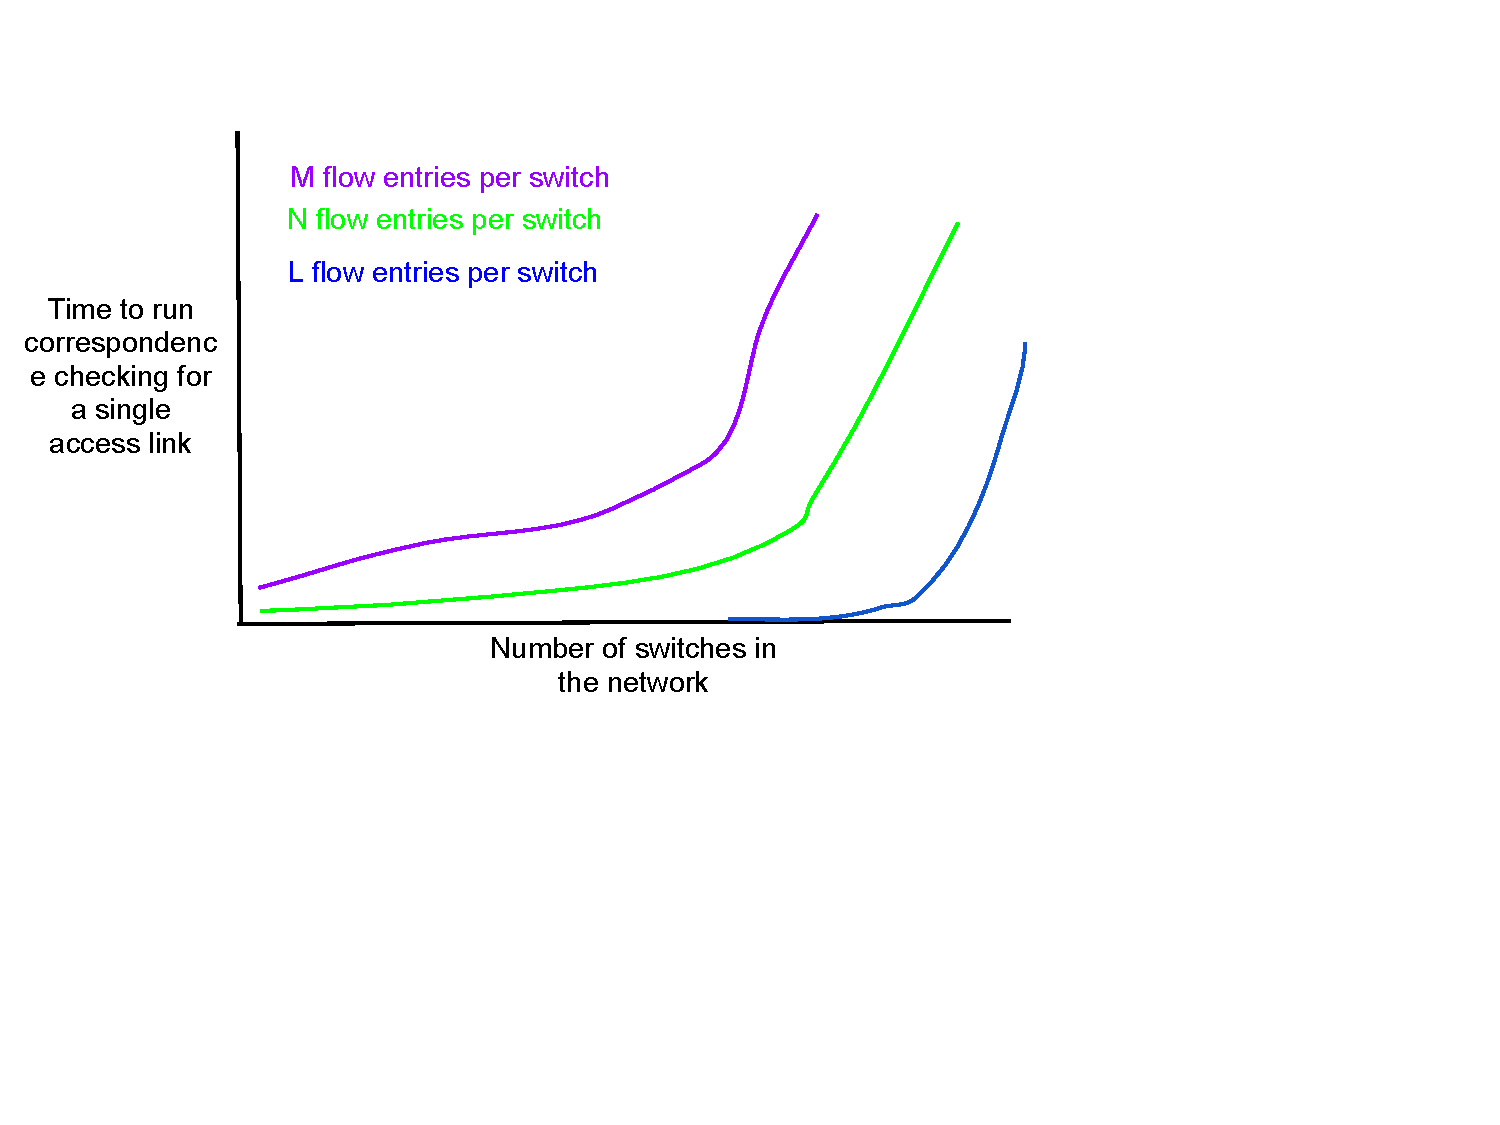
\includegraphics[width=3.25in]{../graphs/mock_hsa_overhead.pdf}
    \caption[]{\label{fig:hsa_runtime} Serial runtime of correspondence
    checking on PORTLAND fat tree networks. Each datapoint consists of
    $x^2/4$ hosts and $5x^2/4$ switches. The serial runtime of correspondence
    checking scales roughly quadratically with the size of the network}
\end{figure}

\noindent{\bf Miscellaneous} \colin{How do you validate the simulator? Is it sufficiently complex to
capture real-world bugs? Conversely, if I catch a failure mode in the
simulator, will my fix work in the production network?}
